\section{DES}

	\begin{frame}
		\begin{center}
			\LARGE{\textcolor{blue}{I giorni nostri: Data Encryption Standard}}
		\end{center}
	\end{frame}

	\subsection{DES}
	
		\begin{frame}
			\frametitle{DES}		
			\begin{itemize}
				\item Sistema crittografico più usato \tblue{attuamente}
				\item Adottato dal \tblue{NIST} (National Institute of Standards and Technology) nel 1977
				\item Si tratta di una \tblue{variante} dei cifrari di Feistel
			\end{itemize}
		\end{frame}
	
		\begin{frame}
			\frametitle{Caratteristiche}		
			\begin{itemize}
				\item Plaintext diviso in blocchi di \tblue{64 bit}
				\item Chiave di \tblue{56 bit}
				\item \tblue{16} round
				\item Dalla chiave \tblue{vengono generate} le 16 sottochiavi da usare una ogni round
			\end{itemize}
		\end{frame}
	
		\begin{frame}
			\frametitle{Funzionamento}	
			\begin{columns}
				\begin{column}{0.4\textwidth}
					\begin{center}
						\begin{figure}
							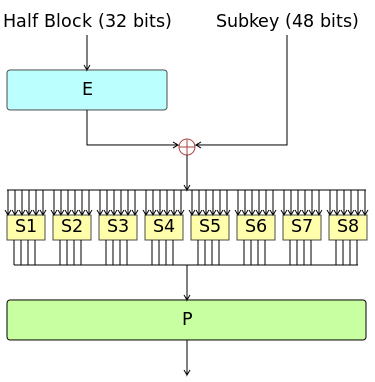
\includegraphics[width=\columnwidth]{img/des}
							\caption{Schema DES}
						\end{figure}
					\end{center}
				\end{column}
				\begin{column}{0.55\textwidth}
					\begin{itemize}
						\item Plaintext (64 bit) diviso a metà (come Feistel)
						\item E \tblue{"espande"} 32 bit portandoli a 48
						\item Viene fatto lo XOR con la \tblue{sottochiave}
						\item Si passa attraverso le \tblue{S-boxes}
						\item I 32 bit che escono dalle S-boxes entrano nella \tblue{P-box} che effettua l'ultima permutazione
					\end{itemize}
				\end{column}		
			\end{columns}		
		\end{frame}
	
		\begin{frame}
			\frametitle{S-boxes}	
			\begin{center}
				\begin{figure}
					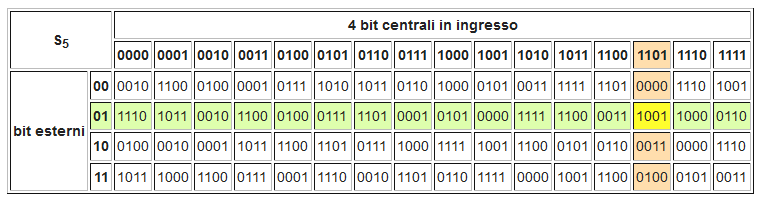
\includegraphics[scale=0.5]{img/desbox}
					\caption{Una S-box}
				\end{figure}
			\end{center}
			\begin{columns}
				\begin{column}{0.5\textwidth}
					\begin{itemize}
						\item \tblue{Input} 6 bit, output 4 bit
						\item Indice di riga i 2 bit più \tblue{esterni}
					\end{itemize}
				\end{column}
				\begin{column}{0.5\textwidth}
					\begin{itemize}
						\item Indice di colonna i 4 bit \tblue{centrali}
						\item \tblue{Output} i 4 bit nella casella selezionata
					\end{itemize}
				\end{column}
			\end{columns}
		\end{frame}
	
		\begin{frame}
			\frametitle{Sottochiavi}	
			\begin{columns}
				\begin{column}{0.3\textwidth}
					\begin{center}
						\begin{figure}
							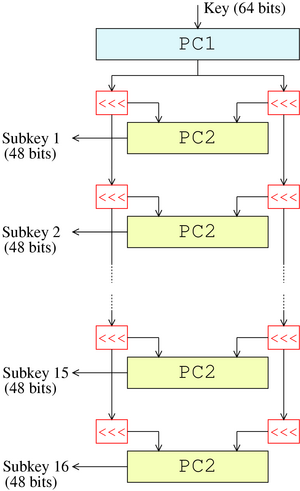
\includegraphics[scale=0.3]{img/deskey}
							\caption{Creazione delle sottochiavi}
						\end{figure}
					\end{center}
				\end{column}
				\begin{column}{0.65\textwidth}
					\begin{itemize}
						\item Selezione di 56 bit della chiave (8 sono di controllo)
						\item Divisi in due metà da 28 bit
						\item Shift a sinistra di 1 o 2 bit a seconda della sottochiave
						\item Selezione di 48 bit
					\end{itemize}
				\end{column}
			\end{columns}	
		\end{frame}
	
		\begin{frame}
			\frametitle{Resistenza}		
			\begin{itemize}
				\item La criptanalisi del DES è quella sulla quale sono state pubblicate \tblue{più informazioni} rispetto ad un qualunque altro algoritmo di cifratura a blocchi
				\item Presenta alcune \tblue{vulnerabilità teoriche} agli attacchi known-plaintext ma, per essere applicate, necessitano di conoscere $\approx 5\cdot10^{11}$ testi in chiaro scelti.
				\item L'\tblue{unico} attacco praticabile resta quello di forza bruta
				\item Attualmente si riesce a trovare la chiave in \tblue{poche ore}
			\end{itemize}
		\end{frame}
	
	\subsection{TripleDES}
	
		\begin{frame}
			\frametitle{Triple DES}		
			\begin{itemize}
				\item 3DES viene standardizzato per \tblue{applicazioni finanziarie} nel 1985
				\item Diventa parte del Data Encryption Standard nel \tblue{1999}
				\item Usa 3 chiavi (\tblue{non necessariamente distinte}) per effettuare tre diverse esecuzioni di DES
			\end{itemize}
		\end{frame}
	
		\begin{frame}
			\frametitle{Schema di funzionamento}		
			\begin{center}
				\begin{figure}
					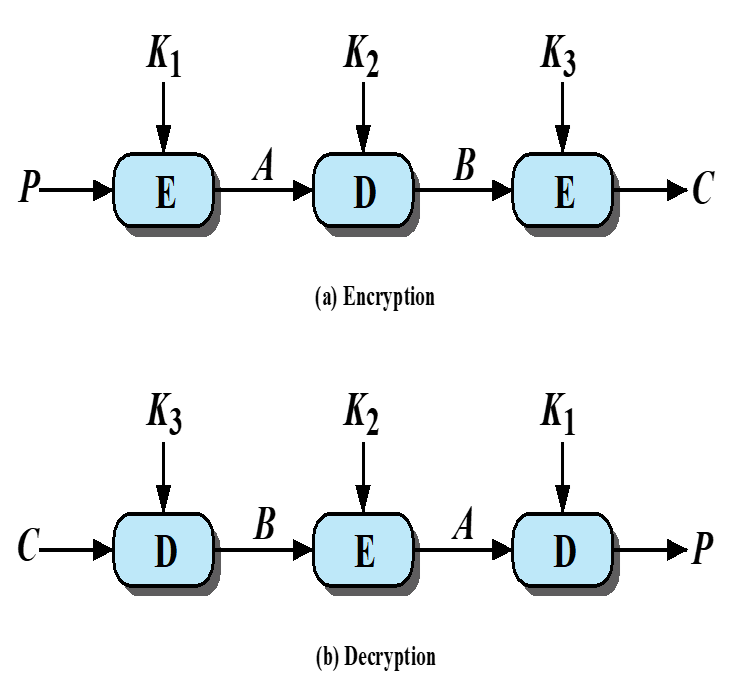
\includegraphics[scale=0.2]{img/tripleDes}
					\caption{Triple DES}
					$C=E(K_3,D(K2,E(K_1,P)))$\\
					$P=D(K_3,E(K2,D(K_1,C)))$
				\end{figure}
			\end{center}
		\end{frame}
	
		\begin{frame}
			\frametitle{Triple DES}		
			\begin{itemize}
				\item Usando sempre la \tblue{stessa} chiave otteniamo DES $$E(K_1,D(K_1,E(K_1,P)))$$
				\item Si possono usare \tblue{due chiavi distinte} e si usano nell'ordine $$E(K_1,D(K_2,E(K_1,P)))$$
				\item Con 3 chiavi distinte si arriva ad una lunghezza di 168 bit e \tblue{si escludono} gli attacchi di forza bruta $$E(K_3,D(K2,E(K_1,P)))$$
			\end{itemize}
		\end{frame}

